\section{Durchführung}
\label{sec:Durchführung}

Für die gesamten Messungen wird die in Abbildung \ref{fig:Durchfuehrung} gezeigte Schaltung verwendet. 
Aufgrund der relativ geringen Signalspannungen müssen diese zusätzlich verstärkt werden. 
\begin{figure}
    \centering
    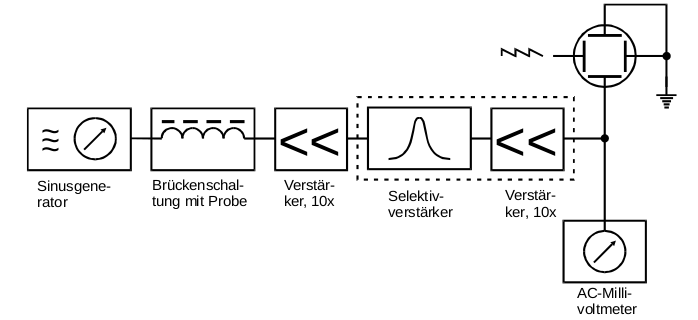
\includegraphics[width=\textwidth]{plots/FinalResult.png}
    \caption{Schaltbild der einzelnen Elemente bei der Messung\cite{Versuchsanleitung}.}
    \label{fig:Durchfuehrung}
\end{figure}
Die Speisespannung wird von einem Sinusgenerator mit Möglichkeit zur Einstellung der Frequenz bezogen. 
Das Modul für die Brückenschaltung, welches bei der Messung verwendet wird, ist in Abbildung \ref{fig:Bruecke} zu sehen.
\begin{figure}
    \centering
    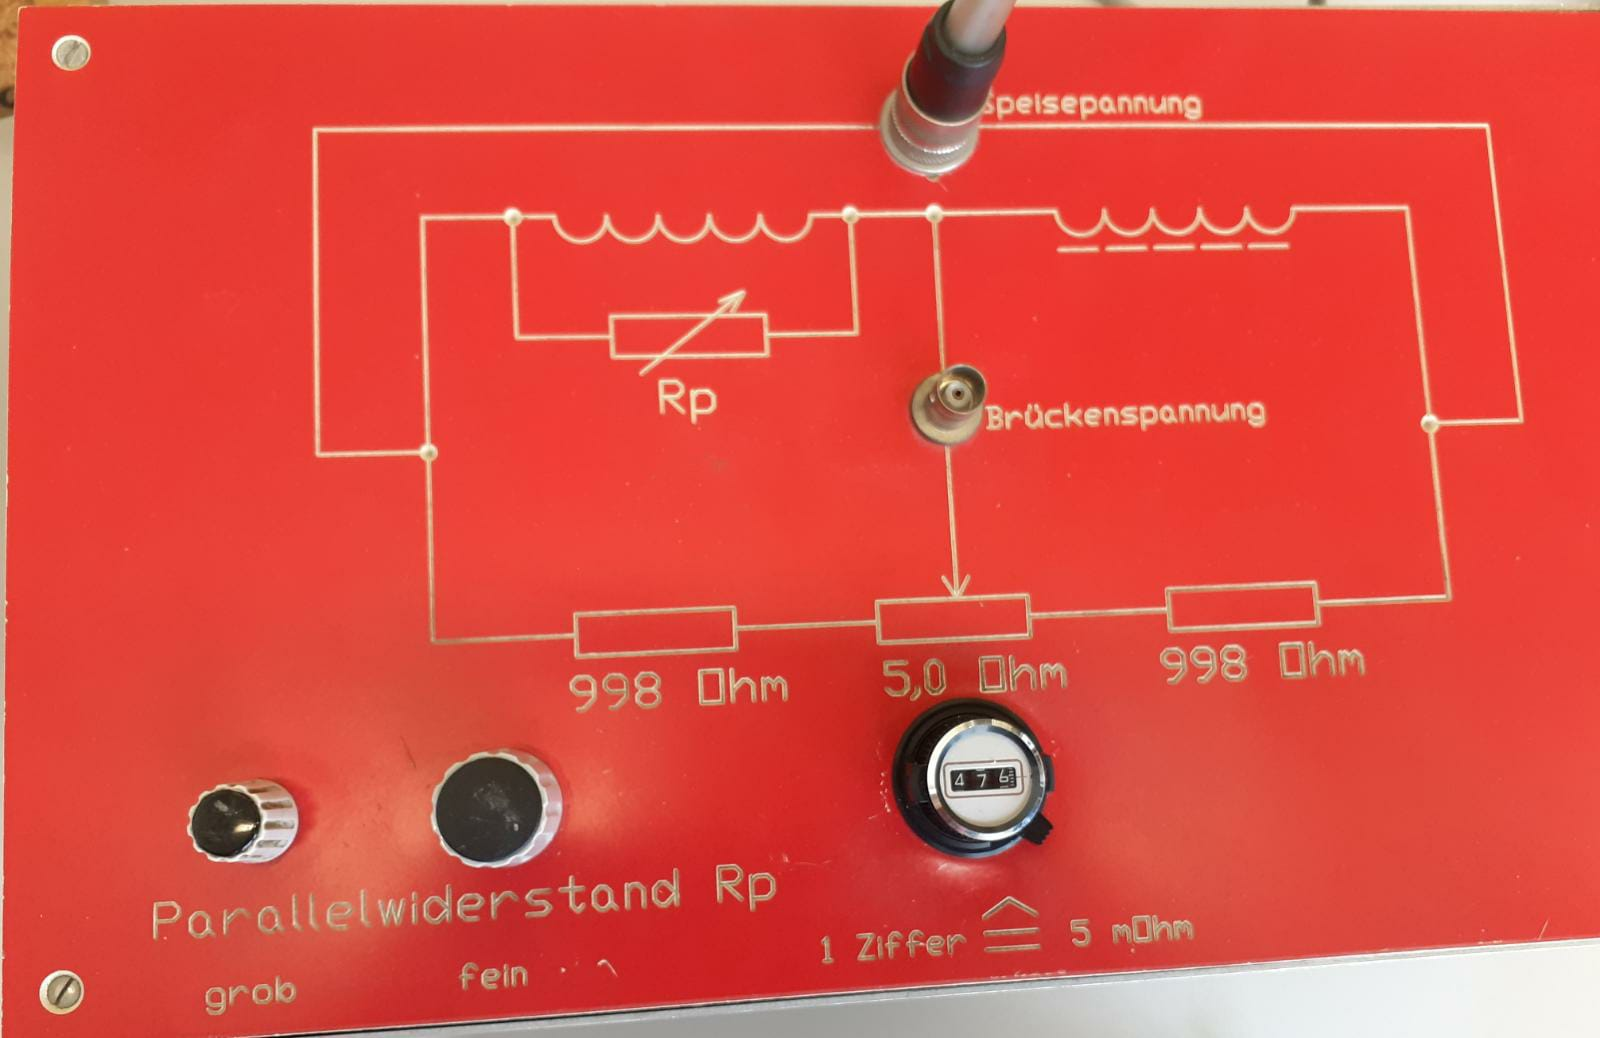
\includegraphics[width=0.6\textwidth]{plots/Durchführung.jpeg}
    \caption{Das bei der Durchführung verwendete Brückenschaltmodul.}
    \label{fig:Bruecke}
\end{figure}
Der Selektivverstärker wird auf eine Güte von $Q=100$ eingestellt.
Nach mehrmaliger Verstärkung des Signals kann zum Schluss die Ausgangsspannung an einem Voltmeter abgelesen werden. 

Vorerst muss die Durchlassfrequenz des Selektivverstärkers möglichst genau bestimmt werden, um die Signalspannung 
bei den folgenden Messungen auf ebendiese Frequenz einstellen zu können.
Hierfür wird in $\SI{1}{\kilo\hertz}$-Schritten der Frequenzbereich $\SI{20}{\kilo\hertz}$-$\SI{40}{\kilo\hertz}$ durchlaufen
und die Ausgangsspannung am Voltmeter aufgezeichnet.
Die von dem Sinusgenerator bezogene Speisespannung beträgt $1\,\mathrm{V}_\text{eff}$.
Die Frequenz, bei der die Ausgangsspannung maximal wird, wird im Folgenden für die Messungen mit Materie verwendet. 

Um eine Veränderung der Induktivität bei Einführung von Materie zu messen, wird zuerst 
die Schaltung ohne jegliche Materie, also nur mit luftgefüllten Spulen, vermessen. 
Der Aufbau wird also entsprechend der Abbildung \ref{fig:Durchfuehrung} realisiert. 

Danach müssen die Brückenwiderstände und der Parallelwiderstand $R_\text{P}$ so eingestellt werden, dass die Ausgangsspannung sich möglichst nah der Null nähert;
die Brückenschaltung wird abgeglichen. 
Die Werte für die Brückenwiderstände und die Brückenspannung werden notiert.

Im Anschluss werden insgesamt drei verschiedene Metalle der Seltenen Erden untersucht.
Hierfür stehen drei Glasröhrchen mit dem entsprechenden Stoff in Pulverform zur Verfügung. 
Da die Suszeptibilität temperaturabhängig ist (vergleiche Gleichung \eqref{eqn:chii}), dürfen die Proben nicht zu 
lange in der Hand gehalten werden. 
Zudem sind die Röhrchen sowie die langen Spulen sehr empfindlich, weshalb diese mit Sorgfalt behandelt werden müssen, um 
Glasbruch oder Vergleichbares zu verhindern. 

Nacheinander werden diese in eine Spule eingeführt und die Brückenwiderstände so reguliert, dass die Brückenspannung 
minimal wird. 
Erneut werden die Werte für die Brückenwiderstände und die -spannung festgehalten. 
